\documentclass[a4paper]{report}

\usepackage[T1]{fontenc}

\usepackage[margin=3.5cm, includeheadfoot]{geometry}
\usepackage{adjustbox}

\usepackage[scale=0.85]{sourcecodepro}

\usepackage{tikz}
\usetikzlibrary{positioning,fit}

\usepackage{booktabs}
\usepackage{listings}

\lstset{%
	language=Eiffel,
	basicstyle=\ttfamily,
	keywordstyle=\bfseries\color{blue},
	showstringspaces=false, tabsize=4,
	deletekeywords={BOOLEAN},
}

\begin{document}

\chapter{Overview}
The etar library provides support for archiving data using the pax/tar format.

\section{Concepts}
\subsection{Archive}
An archive is a series of blocks of size 512 bytes. An entry consists of exactly
one header block, followed by zero or more payload blocks. At the end of the
archive there are two consecutive blocks with all zero bytes.

\begin{figure}[h]
	\begin{center}
		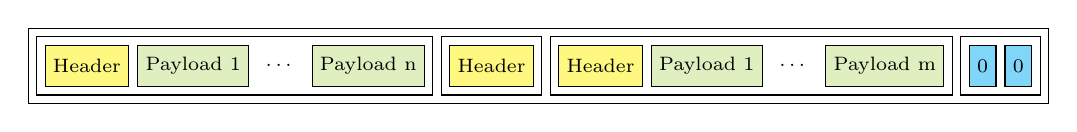
\begin{tikzpicture} [
		every node/.style={inner sep=1mm, node distance=1mm, minimum height=1.5em,
			font=\scriptsize, anchor=west, rectangle},
		entry/.style={draw=black},
		header/.style={draw=black, fill=yellow!50},
		payload/.style={draw=black, fill=green!50!orange!25},
		null/.style={draw=black, fill=cyan!50}
	]
	\node (hdr1) [header] {Header};
	\node (pl11) [payload, right=of hdr1.east] {Payload 1};
	\node (d1) [right=of pl11.east] {\dots};
	\node (pl1n) [payload, right=of d1.east] {Payload n};
	\node (e1) [entry, fit={(hdr1) (pl11) (d1) (pl1n)}] {};

	\node (hdr2) [header, right=of e1.east, xshift=1mm] {Header};
	\node (e2) [entry, fit={(hdr2)}] {};

	\node (hdr3) [header, right=of e2.east, xshift=1mm] {Header};
	\node (pl31) [payload, right=of hdr3.east] {Payload 1};
	\node (d3) [right=of pl31.east] {\dots};
	\node (pl3n) [payload, right=of d3.east] {Payload m};
	\node (e3) [entry, fit={(hdr3) (pl31) (d3) (pl3n)}] {};

	\node (n1) [null, right=of e3.east, xshift=1mm] {0};
	\node (n2) [null, right=of n1.east] {0};

	\node (n) [entry, fit={(n1) (n2)}] {};

	\node (archive) [entry, fit={(e1) (e2) (e3) (n)}] {};

\end{tikzpicture}

	\end{center}
	\caption{Structure of an archive}
\end{figure}

\section{Error Handling}
API still unstable

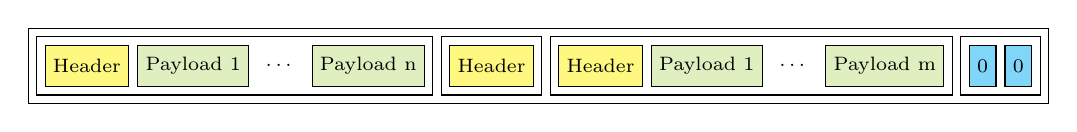
\begin{tikzpicture} [
		every node/.style={inner sep=1mm, node distance=1mm, minimum height=1.5em,
			font=\scriptsize, anchor=west, rectangle},
		entry/.style={draw=black},
		header/.style={draw=black, fill=yellow!50},
		payload/.style={draw=black, fill=green!50!orange!25},
		null/.style={draw=black, fill=cyan!50}
	]
	\node (hdr1) [header] {Header};
	\node (pl11) [payload, right=of hdr1.east] {Payload 1};
	\node (d1) [right=of pl11.east] {\dots};
	\node (pl1n) [payload, right=of d1.east] {Payload n};
	\node (e1) [entry, fit={(hdr1) (pl11) (d1) (pl1n)}] {};

	\node (hdr2) [header, right=of e1.east, xshift=1mm] {Header};
	\node (e2) [entry, fit={(hdr2)}] {};

	\node (hdr3) [header, right=of e2.east, xshift=1mm] {Header};
	\node (pl31) [payload, right=of hdr3.east] {Payload 1};
	\node (d3) [right=of pl31.east] {\dots};
	\node (pl3n) [payload, right=of d3.east] {Payload m};
	\node (e3) [entry, fit={(hdr3) (pl31) (d3) (pl3n)}] {};

	\node (n1) [null, right=of e3.east, xshift=1mm] {0};
	\node (n2) [null, right=of n1.east] {0};

	\node (n) [entry, fit={(n1) (n2)}] {};

	\node (archive) [entry, fit={(e1) (e2) (e3) (n)}] {};

\end{tikzpicture}

\chapter{STORAGE\_BACKEND}
\lstinline;STORAGE_BACKEND; provides a unified interface for different storage
methods an archive could use. Currently the only implementation is
\lstinline;FILE_STORAGE_BACKEND;, providing support for archives that are stored
in a file.

\section{FILE\_STORAGE\_BACKEND}
A \lstinline;FILE_STORAGE_BACKEND; is either created from a file with
\lstinline;make_from_file; or from a filename with
\lstinline;make_from_filename;.

\section{Implementing a Custom STORAGE\_BACKEND}
To implement a custom \lstinline;STORAGE_BACKEND;, one has to implement the
following features:

\subsection{Creation Procedures}
If \lstinline;default_create; is redefined, \lstinline;Precursor; must be
called. Every other creation procedure should call \lstinline;default_create;.

\subsection{open\_read}
\lstinline;open_read;\\
Open backend for read access. Reading should start from the beginning.

\subsection{open\_write}
\lstinline;open_write;\\
Open backend for write access. Writing should start from the beginning.

\subsection{close}
\lstinline;close;\\
Close backend.

\subsection{archive\_finished}
\lstinline;archive_finished: BOOLEAN;\\
Indicate whether the next two blocks contain the end-of-archive indicator
(only zero bytes). The next \lstinline;read_block; calls should not skip these
two blocks but read them again (not necessarily from the backend again, the
implementation is free to chache these blocks).
\lstinline;archive_finished; should return \lstinline;True; too, if an error
occured (or occurs while checking for the end-of-archive indicator), does not
have enough blocks available or if the backend is closed.

\subsection{block\_ready}
\lstinline;block_ready: BOOLEAN;\\
Indicate whether there is a block that can be read with \lstinline;last_block;
\lstinline;False; if an error occured.


\subsection{is\_readable}
\lstinline;is_readable: BOOLEAN;\\
Indicates whether this backend can be read from. If an error occured, this has
to return \lstinline;False;

\subsection{is\_writable}
\lstinline;is_writable: BOOLEAN;\\
Indicates whether this backend can be written to. If an error occured, this has
to return \lstinline;False;

\subsection{is\_closed}
\lstinline;is_closed: BOOLEAN;\\
Indicates whether this backend is closed.

\subsection{read\_block}
\lstinline;read_block;\\
Read next block from backend. If there are not enough bytes for a full block, an
error should be reported.

\subsection{last\_block}
\lstinline;last_block: MANAGED_POINTER;\\
Last block that was read.

\subsection{write\_block}
\lstinline;write_block (block: MANAGED_POINTER);\\
Write \lstinline;block; to the backend (starting from the beginning).

\subsection{finalize}
\lstinline;finalize;\\
Write the end-of-archive indicator and close backend.


\chapter{ARCHIVABLE}
Everything that one wants to add to an archive has to inherit from
\lstinline;ARCHIVABLE;, which provides an interface that \lstinline;ARCHIVE;
uses to write it. The etar library provides two implementations.

\section{FILE\_ARCHIVABLE}
\lstinline;FILE_ARCHIVABLE; allows to archive plain files. A client has to
provide a \lstinline;FILE; for which the \lstinline;FILE_ARCHIVABLE; will be
created.

\section{DIRECTORY\_ARCHIVABLE}
\lstinline;DIRECTORY_ARCHIVABLE; allows to archive a directory (without its
contents!). On creation the client has to provide a \lstiinline;FILE; (!) (for
which \lstinline;is_directory; holds).

\section{Implementing a custom ARCHIVABLE}
To implement a custom \lstinline;ARCHIVABLE;, one has to implement the following
features:



\chapter{UNARCHIVER}

\end{document}
